\documentclass[12pt, a4paper]{article}%Tipo de documento y tamaño de letra%
\usepackage[spanish]{babel}
\usepackage{graphicx}%Para poder insertar graficas%
\usepackage{graphics}
\usepackage{xcolor}
\usepackage{listings}
\lstset{
    language=Matlab,
    basicstyle=\ttfamily\small,
    numbers=left,
    stepnumber=1,
    numbersep=10pt,
    frame=single,
    breaklines=true,
    showstringspaces=false,
    keywordstyle=\color{blue},
    commentstyle=\color{blue!1!black},
    stringstyle=\color{red},
}

\usepackage{amsmath,amssymb}%Insertar unos símbolos matemáticos especiales%
%%%%%%%%%%%%%%%% LA INTEGRAL COMEMIERDA ESA%%

\def\Xint#1{\mathchoice
{\XXint\displaystyle\textstyle{#1}}%
{\XXint\textstyle\scriptstyle{#1}}%
{\XXint\scriptstyle\scriptscriptstyle{#1}}%
{\XXint\scriptscriptstyle\scriptscriptstyle{#1}}%
\!\int}
\def\XXint#1#2#3{{\setbox0=\hbox{$#1{#2#3}{\int}$ }
\vcenter{\hbox{$#2#3$ }}\kern-.6\wd0}}
\def\ddashint{\Xint=}
\def\dashint{\Xint-}

%%%%%%%%%%%%%%%%%%%%%%%%%%%%%%%%%%%%%%%%%%%%

\usepackage{silence}
\WarningFilter{latexfont}{Font shape `T1/ntxtlf/m/up' undefined}
\WarningFilter{latexfont}{Some}
\usepackage{setspace}
%\usepackage{empheq}
\usepackage{multicol}
\usepackage[most]{tcolorbox}
\usepackage{lipsum}
\usepackage{mathrsfs}
\usepackage[T1]{fontenc}
\usepackage{newtxtext,euler}
\let\oldstylenums\oldstyle
\usepackage{array}
\usepackage{layout}
\usepackage{manfnt}
\usepackage{float}
\usepackage{xcolor}
\usepackage{tcolorbox}
\usepackage{lipsum}
\usepackage{tikz}
\usepackage{amsthm}
\usepackage{enumerate}
\usepackage{picinpar}
% Tcolorboxes

\makeatother
\usepackage{thmtools}
\usepackage[framemethod=TikZ]{mdframed}
\mdfsetup{skipabove=1em,skipbelow=1em}

\newcommand{\sqed}{\hfill
\includegraphics[height=2ex]{Graficas/sancoya.png}}

\theoremstyle{definition}
\declaretheoremstyle[
    headfont=\bfseries\sffamily\color{black!70!black}, bodyfont=\normalfont,
    mdframed={
        linewidth=2pt,
        rightline=false,leftline=false, topline=false, bottomline=false,
        linecolor=black, backgroundcolor=black!1!white,
    }
]{thmbox}

\declaretheoremstyle[
    headfont=\bfseries\sffamily\color{black!70!black}, bodyfont=\normalfont,
    numbered=no,
    mdframed={
        linewidth=0pt,
        rightline=false, topline=false, bottomline=false,
        linecolor=black, backgroundcolor=black!2!white,
    },
    qed=\qedsymbol
]{thmproofbox}

\declaretheoremstyle[
    headfont=\bfseries\sffamily\color{black!70!black}, bodyfont=\normalfont,
    numbered=no,
    mdframed={
        linewidth=0pt,
        rightline=false, topline=false, bottomline=false,
        linecolor=black, backgroundcolor=black!2!white,
    },
    qed=\sqed
]{sancoya}


\declaretheorem[style=thmbox, name=Definición]{definition}
\declaretheorem[style=thmbox, numbered=no, name=Ejemplo]{eg}
\declaretheorem[style=sancoya, numbered=no, name=Demostración]{sproof}
\declaretheorem[style=thmbox, name=Proposición]{prop}
\declaretheorem[style=thmbox, name=Teorema, numbered=no]{theorem}
\declaretheorem[style=thmbox, name=Lema]{lemma}
\declaretheorem[style=thmbox, numbered=no, name=Corolario]{corollary}
\declaretheorem[style=thmbox, name=Solución, numbered=no]{solution}


\declaretheorem[style=thmproofbox, name=Demostración]{replacementproof}
\renewenvironment{proof}[1][\proofname]{\vspace{-10pt}\begin{replacementproof}}{\end{replacementproof}}


\declaretheorem[style=thmbox, numbered=no, name=Nota]{note}
\declaretheorem[style=thmbox, numbered=no, ]{temp}




\usepackage{geometry}
 \geometry{
 a4paper,
 total={170mm,245mm},
 left=25mm,
 top=30mm,
 }

\usepackage{bbm}

\begin{document}

\setlength{\parindent}{0cm}
\hoffset-0.46cm
\voffset-1.46cm

\begin{window}[0,l,{
\includegraphics[scale=0.31]{logo.eps}},]
\large\scshape  \hspace{0.4cm}\textsf{Universidad Nacional de Colombia} \\
\textcolor{white}{\tiny.}  \large \hspace{1.5cm} \textsf{Facultad de Ciencias} \\
\textcolor{white}{\tiny.}   \normalsize\hspace{2.2cm}\textsf{Análisis Numérico I}\\
 

\end{window}

\vspace{0.2cm}
\small
\textsf{Mateo Andrés Manosalva Amaris\\
Edgar Santiago Ochoa Quiroga\\
Sergio Alejandro Bello Torres} 
\normalsize
\dotfill
\vspace{0.7cm}

%Ella a mí siempre me trasnocha, yo la pienso a toda hora, pasa por su casa bien sola, deseo que ella sea mi esposa, y anoche yo me presenté en su casa, le dije to' lo que ella a mí me gustaba, ella me dijo "ay papi, qué bonito, échate pa' acá un poquito". Se me fue acercando poco a poquito, con la primera cita ella me dio un besito, me dijo que fuéramos noviecitos y le quité el shorcito. Y la encendí a mondá en la sala de su casa y terminamos en la terraza, yo le pegué su mondaquera en la cama, esa muchacha como gritaba.%
\section*{Problemas}

\subsection*{Problema1}
Un bloque de masa \( m \) desliza bajo la acción de la gravedad por un plano inclinado formando un ángulo \( \theta \) respecto de la horizontal. Se puede demostrar que, si la fuerza de rozamiento \( F_r \) entre el bloque y el plano viene dada por \( F_r = -k m v^2 \) con \( v \) la velocidad del bloque y \( k \) un coeficiente de rozamiento, entonces el tiempo \( T \) requerido para que el bloque recorra una distancia \( D \) partiendo del reposo está relacionado de la forma
\[
e^{kD} = \cosh\left(T \sqrt{k g \sin \theta}\right),
\]
siendo \( g = 9.8 \) la aceleración de la gravedad. Si \( \theta = \frac{\pi}{4} \), \( k = 0.5 \pm 0.1 \) y \( T = 2 \pm 0.2 \), hallar la precisión con la que se conoce \( D \).
\begin{solution}
    Despejando D de la ecuación, se tiene que:
    \[ D=\frac{\ln{\left(\cosh{\left(T\sqrt{kg\sin{\theta}}\right)}\right)}}{k}
    \]
    Tomaremos $D=\varphi(T,k)$, de tal manera que el error relativo venga dado por: 
    \[
    \frac{\phi(\widehat{T},\widehat{k})-\phi(T,k)}{\phi(T,k)}\approx \Delta T\frac{\phi_{T}(T,k)}{\phi(T,k)}+\Delta k\frac{\phi_{k}(T,k)}{\phi(T,k)}
    \]
    Calculando $\phi_{T}$ y $\phi_{k}$ obtenemos:
    \begin{align*}
        \phi_{T}(T,k)&=\sqrt{\frac{g\sin\theta}{k}}\tanh\left(T\sqrt{kg\sin\theta}\right)\\
        \intertext{y}\\
        \phi_{k}(T,k)&=\frac{T\sqrt{kg\sin\theta}\tanh\left(T\sqrt{kg\sin\theta}\right)-2\ln{\left(\cosh{\left(T\sqrt{kg\sin\theta}\right)}\right)}}{2k^2}
    \end{align*}
    Con lo cual la estimación del error nos queda:
    \[
    \frac{\phi(\widehat{T},\widehat{k})-\phi(T,k)}{\phi(T,k)}\approx \Delta T\frac{\sqrt{kg\sin\theta}\tanh\left(T\sqrt{kg\sin\theta}\right)}{\ln\left(\cosh{\left(T\sqrt{kg\sin\theta}\right)}\right)}+\Delta k\left(\frac{T\sqrt{kg\sin\theta}\tanh\left(T\sqrt{kg\sin\theta}\right)}{2k\ln\left(\cosh{\left(T\sqrt{kg\sin\theta}\right)}\right)}-\frac{1}{k}\right)
    \]
    De esta forma, tomando $k=0,5$, $T=2$, $g=9,8$, $\Delta T=0,2$, $\Delta k=0,1$ y sabiendo que $\sin\left(\dfrac{\pi}{4}\right)=\dfrac{\sqrt{2}}{2}$, al calcular $\phi(T,k)$ y estimar el error relativo, obtenemos:
    \begin{align*}
        \phi(T,k)& \approx 6,0605\\
        \intertext{ y el error relativo es}\\
        \frac{\phi(\widehat{T},\widehat{k})-\phi(T,k)}{\phi(T,k)}\approx 0,2\times&\frac{1,8592}{3,0302}+0,1\times\left(\frac{3,7185}{3,0302}-2\right)\approx 0,0454
    \end{align*}
    Así, obtenemos un error relativo de $4,54\times10^{-2}\leq5\times10^{-2}$, lo cual significa que solo conocemos $D$ con una precisión de una cifra significativa.
    \end{solution}
\subsection*{Problema2}
Utilizando el método de redondeo.

\begin{itemize}
    \item[(a)] Hallar el número de máquina más próximo a 125.6 y a 126 si trabaja con
    \begin{itemize}
        \item Base 10 y mantisa de 2 dígitos.
        \begin{solution}
            Para usar el método de redondeo, verificamos que para truncar 125,6 a 2 dígitos, el tercer dígito es $5\geq\frac{10}{2}$, por lo tanto obtenemos 130 y la representación de 125,6 en punto flotante es:
            \[
            fl(125,6)=1.3\times10^{2}
            \]
            De manera análoga, para 126, vemos que $6\geq\frac{10}{2}$, así:
            \[
            fl(126)=1.3\times10^{2}
            \]
            De donde concluimos que 130 es el número de máquina más próximo a 125,6 y 126.
        \end{solution}
        \item Base 2 y mantisa de 8 dígitos.
        \begin{solution}
            Primero, convertimos 125,6 y 126 a base 2; Para convertir 125 a base 2 tenemos:
            \begin{center}
            \renewcommand{\arraystretch}{1.2}
                \begin{tabular}{|c|c|c|}\hline
                División & Cociente & Residuo\\ \hline
                125$\div$2 & 62 & 1 \\ 
                62$\div$2 & 31 & 0 \\ 
                31$\div$2 & 15 & 1 \\
                15$\div$2 & 7 & 1 \\
                7$\div$2 & 3 & 1 \\
                3$\div$2 & 1 & 1 \\
                1$\div$2 & 0 & 1\\ \hline
                \end{tabular}
            \end{center}
            Ahora, convertimos 0,6 a base 2:
            \begin{center}
                \renewcommand{\arraystretch}{1.2}
                \begin{tabular}{|c|c|c|}\hline
                   Producto & Resultado & Parte entera \\ \hline
                    0.6$\times$2 & 1.2 & 1 \\
                    0.2$\times$2 & 0.4 & 0 \\
                    0.4$\times$2 & 0.8 & 0 \\
                    0.8$\times$2 & 1.6 & 1 \\
                    0.6$\times$2 & 1.2 & 1\\
                    $\vdots$ & $\vdots$ & $\vdots$ \\ \hline
                \end{tabular}
            \end{center}
            Así, 125,6 en binario es:
            \[
            (125,6)_{10}=(1111101,\overline{10011})_{2}
            \]
            Ya que en el sistema binario, el único digito diferente de 0 es 1, podemos representar el número con 9 dígitos, de esta forma, observamos que el décimo dígito de esta representación es 0, por lo tanto truncamos a 9 dígitos y así obtenemos
            \[
            fl(125,6)=1,11110110_{2}\times2^{6}
            \]
            Es decir, el número de máquina más próximo a 125,6 en base 2 y mantisa de 8 dígitos es 
            \[
        \left(1+\frac{1}{2}+\frac{1}{2^{2}}+\frac{1}{2^{3}}+\frac{1}{2^{4}}+\frac{0}{2^{5}}+\frac{1}{2^{6}}+\frac{1}{2^{7}}+\frac{0}{2{8}}\right)\times 2^{6}=125,5 
            \]
            
            Ahora convertimos 126 a base 2:
            \begin{center}
            \renewcommand{\arraystretch}{1.2}
                \begin{tabular}{|c|c|c|}\hline
                División & Cociente & Residuo\\ \hline
                126$\div$2 & 63 & 0 \\ 
                63$\div$2 & 31 & 1 \\ 
                31$\div$2 & 15 & 1 \\
                15$\div$2 & 7 & 1 \\
                7$\div$2 & 3 & 1 \\
                3$\div$2 & 1 & 1 \\
                1$\div$2 & 0 & 1\\ \hline
                \end{tabular}
            \end{center}
            Por lo tanto
            \[
            (126)_{10}=(1111110)_{2}
            \]
            Este numero es de 7 dígitos, por lo tanto se puede representar exactamente en punto flotante:
            \[
            fl(126)=1,11111000_{2}\times2^{6}
            \]
            luego el número de maquina más próximo a 126 es 126.
            
        \end{solution}
    \end{itemize}
    \item[(b)] Verificar para \( x = 125.6 \) la cota para el error relativo
    \[
    \left|\frac{x - \text{fl}(x)}{x}\right| \leq \epsilon
    \]
    si \( \epsilon = \frac{1}{2} \beta^{1-d} \) donde \( \beta \) es la base y \( d \) la longitud de la mantisa.
    \begin{solution}
        Para la representación en base 10 y mantisa de 2 dígitos, el error relativo es:
        \[
        \left|\frac{125,6-130}{125,6}\right|=0.035<\frac{1}{2}\times10^{1-2}=0,05
        \]
        De manera similar, calculamos el error para base 2 y mantisa de 8 dígitos
        \[
        \left|\frac{125,6-125,5}{125,6}\right|\approx 0,000796<\frac{1}{2}\times2^{1-8}=2^{-8}=0,00390625
        \]
        En ambos casos, verificamos que se cumple la cota del error.
    \end{solution}
    \item[(c)] ¿Cuál es, en cada caso, el valor que da la máquina como resultado de las operaciones \( 126 + 126.5 \) y \( 126 - 125.6 \)? ¿Cuál es el error relativo de estos resultados?
    \begin{solution}
        \begin{itemize}
            \item Para base 10 y mantisa de 2 dígitos se tiene:
            \begin{align*}
                fl(126+126,5)&=fl(fl(126)+fl(126,5))\\
                &=fl(1,3\times10^2+1,3\times10^2)\\
                &=fl(2,6\times10^2)\\
                &=2,6\times10^2\\
                &=260
            \end{align*}
            Sin embargo 126+126,5=252,5, por lo tanto el error relativo de este resultado es:
            \[
            \left|\frac{252,5-260}{252,5}\right|\approx 0,0297
            \]
            Calculemos ahora $fl(126-125,6)$
            \begin{align*}
                fl(126-125,6)&=fl(fl(126)-fl(125,6))\\
                &=fl(1,3\times10^2-1,3\times10^2)\\
                &=fl(0)\\
                &=0
            \end{align*}
            El error relativo es, entonces:
            \[
            \left|\frac{0,4-0}{0,4}\right|= 1
            \]
            Aquí podemos ver que debido a que el sistema de punto flotante representa dos números distintos con el mismo número, aunado a la pequeña cantidad de dígitos de la mantisa, el error llega a propagarse de tal manera que al restar dos números cercanos se obtiene un error relativo del 100\%, lo cual significa que en algunos casos, no podemos conocer ninguna cifra significativa al efectuar la resta de dos números de máquina.
            \item Base 2 y mantisa de 8 dígitos. 
            
            Para convertir 126,5 a binario usaremos que $(126)_{10}=(1111110)_{2}$ y $(0,5)_{10}=(0,1_{2})$, de esta manera $(126,5)_{10}=(1111110,1)_{2}$ y su representación en punto flotante es $fl(126,5)=1,11111010_{2}\times2^6$. Así, al efectuar 126+126,5 tenemos:
            \begin{align*}
                fl(126+126,5)&=fl(fl(126)+fl(126,5))\\
                &=fl(1,11111000_{2}\times2^{6}+1,1111101_{2}\times2^{6})\\
                &=fl(11,1111001_{2}\times2^{6})\\
                &=1,11111001_{2}\times2^{7}
            \end{align*}
            Es decir:
            \[
            \left(1+\frac{1}{2}+\frac{1}{2^{2}}+\frac{1}{2^{3}}+\frac{1}{2^{4}}+\frac{1}{2^{5}}+\frac{0}{2^{6}}+\frac{0}{2^{7}}+\frac{1}{2^{8}}\right)\times2^{7}=252,5
            \]
            Hallamos entonces el error relativo
            \[
            \left|\frac{252,5-252,5}{252,2}\right|= 0
            \]
            Calculemos ahora 126-125,6:
            \begin{align*}
                fl(126-125,6)&=fl(fl(126)-fl(125,6))\\
                &=fl(1,11111000_{2}\cdot2^{6}-1,11110110_{2}\cdot2^{6})\\
                &=1,0000000_{2}\cdot2^{-1}
            \end{align*}
            Es decir $fl(126-125,6)=0,5$, luego el error relativo es:
            \[
            \left|\frac{0,6-0,5}{0,6}\right|=0,1\overline{6}
            \]
        \end{itemize}
    \end{solution}
\end{itemize}

\subsection*{Problema3}
Suponga que una compañía de computadores está desarrollando un nuevo sistema de punto flotante para usarlo con sus máquinas. Ellos necesitan su ayuda para responder unas preguntas acerca de su sistema. Siguiendo la terminología descrita en clase, el sistema de punto flotante de la compañía se especifica por \( (\beta, t, L, U) \). Usted debe suponer que:

\begin{itemize}
    \item Todos los valores de punto flotante son normalizados (excepto la representación de punto flotante de cero).
    \item Todos los dígitos en la mantisa de un valor de punto flotante son almacenados explícitamente.
    \item El cero se representa con una mantisa y exponente de ceros.
\end{itemize}

Preguntas:
\begin{itemize}
    \item[(a)] ¿Cuántos valores diferentes de punto flotante no negativos pueden representarse por medio de este sistema de punto flotante?
    \begin{solution}
    Recordemos que en general la representación de punto flotante esta dada por
    $$fl(x)=\pm\left(d_0+\frac{d_1}{\beta}+\frac{d_2}{\beta^2}+\cdots+\frac{d_{t-1}}{\beta^{t-1}}\right)\beta^e=\pm(d_0.d_1d_2\dots d_{t-1})\beta^e$$
     Como son los no negativos y los valores del punto flotante están normalizados, Procedamos primero con los positivos, como todos los valores están normalizados, el primer dígito de la representación tiene que ser diferente de 0, es decir, $1\leq d_0\leq \beta-1,$ luego para $d_i$ con $1\leq i\leq t-1$, como estos no tienen restricción podemos tomarlos tal que $0\leq d_0\leq \beta-1.$ Por lo que de momento, por el principio fundamental del conteo tenemos $(\beta-1)(\beta)^{t-1}$ valores diferentes. Note que decimos de momento ya que no hemos considerado los posibles exponentes. Ahora tomando $e$ un posible exponente, sabemos que $L\leq e\leq U$, luego la cantidad de posibles exponentes para cada uno de los valores encontrados seria $U-L+1.$ Así concluimos que la cantidad de valores no negativos diferentes en este sistema de punto flotante es
     $$(\beta-1)(\beta)^{t-1}(U-L+1)+1=.$$
     Note que ese mas 1 del final es añadido para contar el caso particular del 0, que es el único que tiene una mantisa y exponente de ceros.
    \end{solution}
    \item[(b)] La misma pregunta para el caso \( (\beta, t, L, U) = (8, 5, -100, 100) \), el cual la compañía está contemplando en particular.
    \begin{solution}
        Como hallamos en el numeral anterior una formula para un sistema de punto flotante arbitrario, aquí basta simplemente con reemplazar los respectivos valores, es decir
        \begin{align*}
           (\beta-1)(\beta)^{t-1}(U-L+1)+1&=(8-1)8^{(5-1)}(100-(-100)+1)+1\\
           &=7\cdot 8^4\cdot201+1\\
           &=5763073.
        \end{align*}
    \end{solution}
    \item[(c)] ¿Cuál es el valor aproximado (en base 10) del número más grande y el número positivo más pequeño que pueden ser representado en este sistema de punto flotante?
    \begin{solution}
    \begin{itemize}
        \item Primero responderemos la pregunta de cual es el numero mas grande. Tenemos que tal numero seria uno donde cada $d_i=\beta-1$ y nuestro $e=U$, así para el sistema particular tenemos que ese numero es
        $$x=(7.7777)8^{100}.$$
        Ahora si lo vemos en representación decimal tenemos que
        $$x=\left(7+\frac{7}{8}+\frac{7}{8^2}+\frac{7}{8^3}+\frac{7}{8^4}\right)8^{100}\approx 1,62957\times10^{91}.$$
        \item Ahora el numero mas pequeño positivo es cuando tenemos que $d_0=1$, mientras que $d_i=0$ para los demás, esto ya que esta normalizado, y consideramos $e=L$. Para nuestro caso particular tenemos que 
        $$y=(1.0000)8^{-100}=\left(1+\frac{0}{8}+\frac{0}{8^2}+\frac{0}{8^3}+\frac{0}{8^4}\right)8^{-100}\approx4,90909\times 10^{-91}.$$  
    \end{itemize}   
    \end{solution}
    \item[(d)] Para el caso general, demuestre que los errores relativos producidos por realizar truncamiento y redondeo son
    \[
    \left|\frac{\text{fl}(x) - x}{x}\right| \leq
    \begin{cases}
        \beta^{1-t} & \text{cuando se efectúa truncamiento}, \\
        \frac{1}{2} \beta^{1-t} & \text{cuando se efectúa redondeo}.
    \end{cases}
    \]
\end{itemize}
\begin{sproof}
    La prueba la tenemos que dividir en el caso del truncamiento y el caso del redondeo. Primero consideremos el caso del truncamiento. Tenemos que la expansión decimal de un numero $x>0,$ en un sistema de punto flotante arbitrario es
    $$x=\left(d_0+\frac{d_1}{\beta}+\frac{d_2}{\beta}+\cdots+\frac{d_{t-1}}{\beta^{t-1}}+\frac{d_t}{\beta^{t}}+\frac{d_{t+1}}{\beta^{t+1}}+\cdots\right)\beta^e=(d_0.d_1d_2\dots d_{t-1}d_{t}d_{t+1}\dots)\beta^e.$$
    Luego si realizamos el truncamiento en el termino $t-1$, es decir, hacemos $0$ los $d_i$ cuando $i>t-1.$ tenemos que
    $$fl(x)=\left(d_0+\frac{d_1}{\beta}+\frac{d_2}{\beta}+\cdots+\frac{d_{t-1}}{\beta^{t-1}}\right)\beta^e.$$
    Ahora note que si consideramos el error absoluto, obtenemos que
    \begin{align*}
        |fl(x)-x|&=\left|\left(-\frac{d_t}{\beta^{t}}-\frac{d_{t+1}}{\beta^{t+1}}-\cdots\right)\beta^e\right|\\
        &=\left(\frac{d_t}{\beta^{t}}+\frac{d_{t+1}}{\beta^{t+1}}+\cdots\right)\beta^e\\
        &=\left(d_t+\frac{d_{t+1}}{\beta}+\cdots\right)\frac{\beta^e}{\beta^t}\\
        &\leq \beta^{1+e-t}
    \end{align*}
    Note que como $d_i\leq \beta$ para todo $i,$ ese ultimo paso para acotar es valido. Ahora note que como $x>0,$ tenemos que $|x|\geq d_0\beta^e\geq \beta^e.$ En efecto, ya que como el sistema esta normalizado, necesariamente $d_0\geq 1$ y ademas el numero $d_0$ seguido de ceros es siempre menor que $d_0$ seguido de cualquier cadena de dígitos permitida. Así tenemos que $\dfrac{1}{|x|}\leq \dfrac{1}{\beta^e}.$ Multiplicando en la anterior desigualdad obtenida tenemos que
    $$\left|\frac{fl(x)-x}{x}\right|\leq \frac{\beta^{1+e-t}}{\beta^e}=\beta^{1-t}.$$

    Ahora consideremos el caso donde redondeamos. Note que podemos asumir que $d_t\geq \dfrac{\beta}{2},$ ya que en caso contrario no hay redondeo y simplemente es un truncamiento. En este caso nuestra aproximación es
    $$fl(x)=\left(d_0+\frac{d_1}{\beta}+\frac{d_2}{\beta}+\cdots+\frac{d_{t-1}+1}{\beta^{t-1}}\right)\beta^e=(d_0.d_1d_2\dots (d_{t-1}+1))\beta^e.$$
    Luego si consideramos nuevamente el error absoluto, obtenemos 
    \begin{align*}
    |fl(x)-x|&=|(0.\underbrace{0\dots 0}_{t-1 veces}(\beta-1-d_t)(\beta-1-d_{t+1})\dots)\beta^e|\\
        &=((\beta-1-d_t).(\beta-1-d_{t+1})\dots)\beta^{e-t}\\
        &\leq \frac{1}{2}\beta\beta^{e-t}=\frac{\beta^{1+e-t}}{2}.
    \end{align*}
    En efecto, ya que como $d_t\geq \dfrac{\beta}{2},$ tenemos que $\beta-1-d_t\leq\beta-1-\dfrac{\beta}{2}=\dfrac{\beta}{2}-1\leq \dfrac{\beta}{2}.$ Como el $x$ sigue siendo el mismo del anterior caso, seguimos teniendo que $\dfrac{1}{|x|}\leq \dfrac{1}{\beta^e}.$ Procediendo de la misma manera obtenemos
    $$\left|\frac{fl(x)-x}{x}\right|\leq \frac{\beta^{1+e-t}}{2\beta^e}=\frac{1}{2}\beta^{1-t}.$$
    Note que el caso cuando $x=0$ no es necesario revisarlo ya que la representación es idéntica, mientras que el caso $x<0$ como estamos trabajando dentro de un valor absoluto es aplicar el mismo razonamiento. De esta manera hemos demostrado que
    \[
    \left|\frac{\text{fl}(x) - x}{x}\right| \leq 
    \begin{cases}
        \beta^{1-t} & \text{cuando se efectúa truncamiento}, \\
        \frac{1}{2} \beta^{1-t} & \text{cuando se efectúa redondeo}.
    \end{cases}
    \]
    
\end{sproof}

\subsection*{Problema4}
Considere la expansión de Taylor para la función exponencial
\[
e^x = 1 + x + \frac{x^2}{2!} + \frac{x^3}{3!} + \dots = \sum_{i=0}^{\infty} \frac{x^i}{i!} = \lim_{N \to \infty} S(x, N)
\]
donde \( S(x, N) \) es la suma parcial con \( N + 1 \) términos.

\begin{itemize}
    \item[(a)] Escriba un programa que grafique el error relativo de la suma, \( \dfrac{|S(x, N) - e^x|}{e^x} \) versus \( N \) (hasta \( N = 60 \)) para un valor dado de \( x \). Pruebe su programa para \( x = 10, 2, -2 \) y \( -10 \). De las gráficas, explique por qué ésta no es una buena manera para evaluar \( e^x \) cuando \( x < 0 \).

    \begin{solution}

    Implementamos en Python un código que grafica el error relativo de la suma parcial de Taylor, obtuvimos el resultado

    \begin{figure}[H]
        \centering
        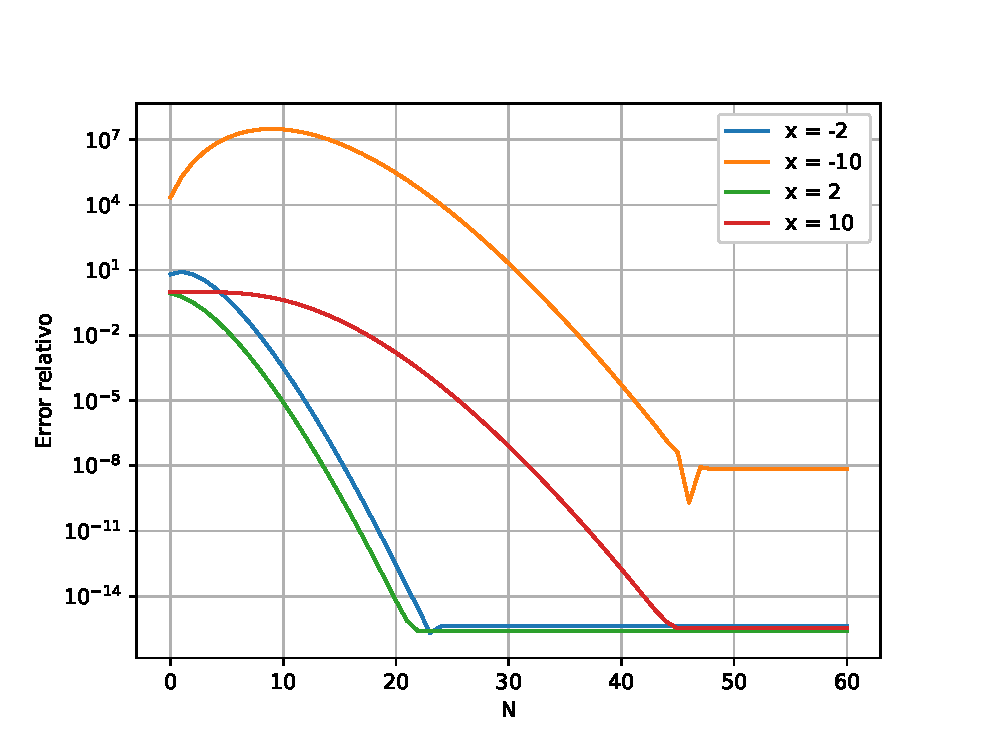
\includegraphics[width=0.75\linewidth]{Gráficas/AN-T1-P4A.eps}
        \caption{Error relativo}
        \label{coyo4}
    \end{figure}

En la gráfica se evidencia que el error aumenta cuando los valores de $x$ son negativos, note que si $x$ es negativo entonces reescribimos la expresión como $e^{-x}$ con $x>0$, de esto se sigue que
\[
e^{-x} = 1 -x + \frac{x^2}{2!} - \frac{x^3}{3!} + \dots = \sum_{i=0}^{\infty} \frac{(-1)^ix^i}{i!} = \lim_{N \to \infty} \dfrac{1}{S(x,N)},
\]

como al calcular el error necesitamos aproximar este término, entonces al truncar la serie alternante obtenemos resultados que oscilan alrededor del 0, por lo que la expresión $1/S(x,N)$ toma valores grandes, en cambio si $x$ es positivo nuestra serie truncada se aleja cada vez más de 0.
    \end{solution}
    
    \item[(b)] Modifique su programa tal que use la identidad \( e^x = \dfrac{1}{e^{-x}} = \dfrac{1}{S(-x, \infty)} \) para evaluar la función exponencial cuando \( x \) es negativa. Explique por qué esta técnica funciona mejor.

\begin{solution}
    Para este caso obtuvimos la gráfica del error

    \begin{figure}[H]
        \centering
        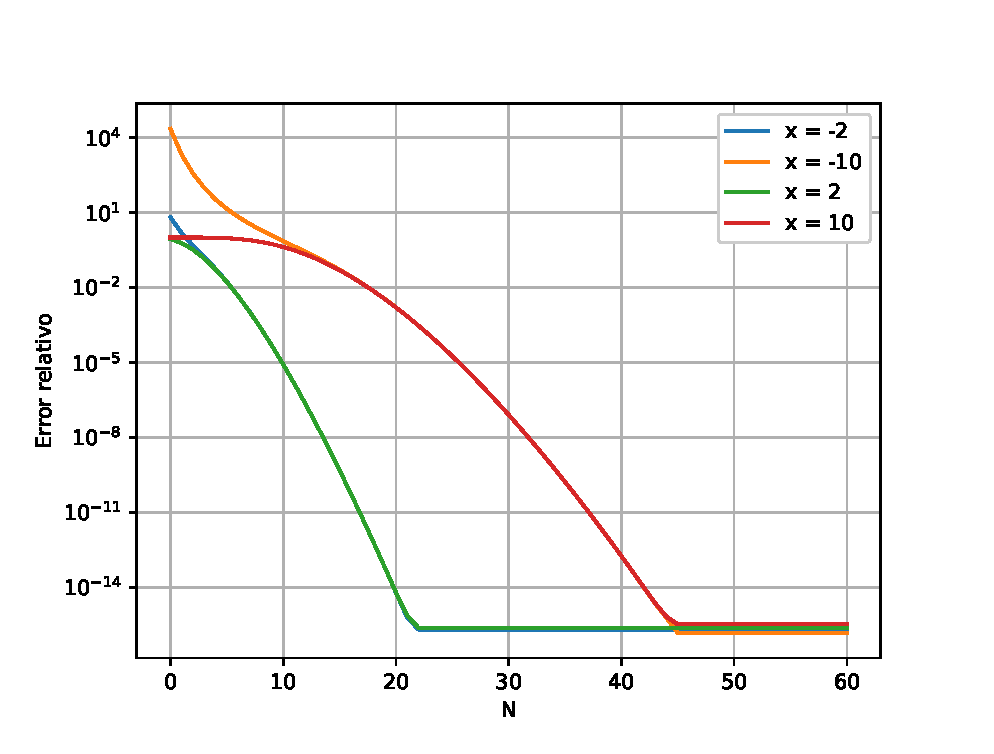
\includegraphics[width=0.75\linewidth]{Gráficas/AN-T1-P4B.eps}
        \caption{Error relativo}
        \label{coyo4B}
    \end{figure}

    Esta técnica funciona mejor ya que si $x<0$, entonces $-x>0$ y por lo tanto al calcular 

    $$e^x=\dfrac{1}{e^{-x}}\quad x<0,$$

    el término $-x$ es positivo y podemos aproximar de manera adecuada $e^{-x}$ por $S(-x,N)$ como consecuencia del numeral anterior ya la serie no es alternante.
\end{solution}
    
\end{itemize}

\subsection*{Problema5}
\begin{itemize}
    \item[(a)] De manera similar a la desarrollada en clase, deduzca que una aproximación de \( f'(x_0) \) es
    \[
    \dfrac{f(x_0 + h) - f(x_0 - h)}{2h}.
    \]
    Muestre que esta aproximación tiene un error de \( O(h^2) \). Más precisamente, el primer término del error es \( -\dfrac{h^2}{6} f'''(x_0) \) cuando \( f'''(x_0) \neq 0 \).

\begin{proof}
Por el teorema de Taylor tenemos que

$$
f\left(x_0+h\right)=f\left(x_0\right)+h f^{\prime}\left(x_0\right)+\frac{h^2}{2}  f^{\prime \prime}\left(x_0\right)+\frac{h^3}{6} f^{\prime \prime \prime}\left(x_0\right)+\cdots,
$$

además
    
$$
f\left(x_0-h\right)=f\left(x_0\right)-h f^{\prime}\left(x_0\right)+\frac{h^2}{2}  f^{\prime \prime}\left(x_0\right)-\frac{h^3}{6} f^{\prime \prime \prime}\left(x_0\right)+\cdots,
$$

luego el error de aproximación de $f^{\prime}\left(x_0\right)$ por la expresión planteada no considera los términos pares de la expansión de Taylor ya que tienen el mismo signo y se cancelan al realizar la resta como sigue

$$
f\left(x_0+h\right)-f\left(x_0-h\right)=2 h f^{\prime}\left(x_0\right)+\frac{h^3}{6} f^{\prime \prime \prime}\left(x_0\right)+\frac{h^3}{6} f^{\prime \prime \prime}\left(x_0\right)+O(h^5),
$$

así

$$
\begin{aligned}
\frac{f\left(x_0+h\right)-f\left(x_0-h\right)}{2 h} & =f^{\prime}\left(x_0\right)+\frac{ 2h^3}{2h6} f^{\prime \prime \prime}\left(x_0\right)+\cdots \\
& =f^{\prime}\left(x_0\right)+\frac{h^2}{6} f^{\prime \prime \prime}\left(x_0\right)+\cdots,
\end{aligned}
$$

se sigue que


$$\left|\frac{f\left(x_0+h\right)-f\left(x_0-h\right)}{2 h}-f^{\prime}(x_0)\right|\leq \frac{h^2}{6} f^{\prime \prime \prime}\left(x_0\right)$$

\end{proof}
    
    \item[(b)] Adapte el programa de Matlab hecho en clase para visualizar el comportamiento del error de aproximación a medida que el paso \( h \) decrece desde \( h = 10^{-1}, \dots, 10^{-16} \).

\begin{solution}
        Implementamos el siguiente código:\\

        \newpage

\begin{lstlisting}
x0 = 1.2;       
f0 = sin(x0);       
fp = cos(x0);     
i = -16:0.5:-1;
h = 10.^i;
err_centrada = abs(fp - (sin(x0 + h) - sin(x0 - h)) ./ (2 * h));
d_err_centrada = fp / 6 * h.^2;
loglog(h, d_err_centrada, 'r-.', h, err_centrada, 'b-*', 'LineWidth', 2);
xlabel('h', 'fontsize', 16);
ylabel('Error Absoluto', 'fontsize', 14);
legend('Error de truncamiento', 'Diferencias finitas', 'location', 'southwest');
grid on;
\end{lstlisting}


con lo que obtuvimos la gráfica

\begin{figure}[H]
    \centering
    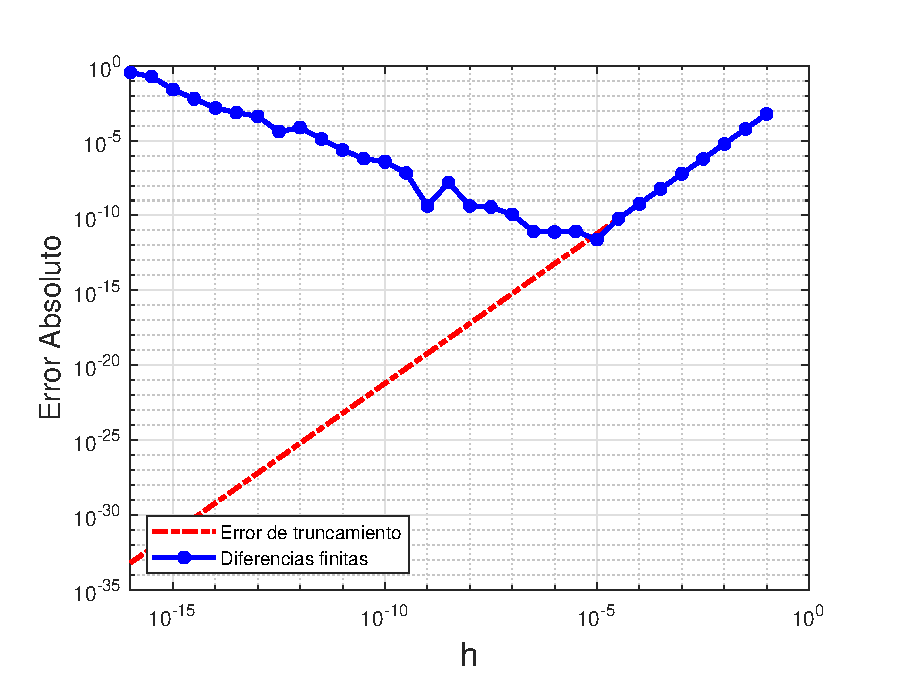
\includegraphics[width=0.75\linewidth]{Gráficas/P5-1.eps}
    \caption{P5-1}
    \label{fig:bluelabel}
\end{figure}
    
\end{solution}

    \item[(c)] Muestre que
    \[
    f'(x_0) = \dfrac{-f(x_0 + 2h) + 8f(x_0 + h) - 8f(x_0 - h) + f(x_0 - 2h)}{12h} + O(h^4)
    \]
    De nuevo adapte su programa para visualizar el comportamiento del error de aproximación a medida que el paso \( h \) decrece desde \( h = 10^{-1}, \dots, 10^{-16} \).
\end{itemize}

\begin{proof}
    De manera análoga al numeral a) tenemos que
    
$$
8f\left(x_0+h\right)-8f\left(x_0-h\right)=16 h f^{\prime}\left(x_0\right)+16\frac{h^3}{6} f^{\prime \prime \prime}\left(x_0\right)+ \dfrac{8h^5}{60}f^{(5)}(x_0)+O(h^6),
$$

por otro lado

$$\begin{aligned}
 -f(x_0+2 h)&=-f\left(x_0\right)-2h f^{\prime}\left(x_0\right)-\frac{4 h^2}{2} f^{\prime \prime}\left(x_0\right)-\frac{8 h^3}{6} f^{\prime\prime \prime}\left(x_0\right)-\dfrac{16h^4}{24}f^{(4)}(x_0)-\dfrac{32h^5}{120}f^{(5)}(x_0)\\
&\hspace{0.5cm}+O\left(h^6\right),\\
f(x_0-2 h)&=f\left(x_0\right)-2 h f^{\prime}\left(x_0\right)+\frac{4 h^2}{2}f^{\prime\prime}(x_0)-\frac{8 h^3}{6} f^{\prime \prime \prime}\left(x_0\right)+\dfrac{16h^4}{24}f^{(4)}(x_0)-\dfrac{32h^5}{120}f^{(5)}(x_0)\\
&\hspace{0.5cm}+O\left(h^6\right),
\end{aligned}
$$

sumando estas expresiones obtenemos que 

$$8f\left(x_0+h\right)-8f\left(x_0-h\right)-f(x+2h)+f(x_0+2h)=12hf^{\prime}(x_0)-\dfrac{2h^5}{5}f^{(5)}(x_0)+O(h^6).$$

En efecto 

\begin{align*}
     \dfrac{-f(x_0 + 2h) + 8f(x_0 + h) - 8f(x_0 - h) + f(x_0 - 2h)}{12h}&=\dfrac{12hf^{\prime}(x_0)+O(h^5)}{12h}\\
     =f^{\prime}(x_0)+O(h^4),
\end{align*}

de hecho no era necesario controlar el error de de la quinta derivada para concluir este primer numeral, pero lo hicimos para poder adaptar el programa y visualizar de manera más precisa el error de truncamiento, obtenemos que el primer término de error es

$$\dfrac{h^4}{30}f^{\prime\prime\prime\prime\prime}(x_0)$$
\end{proof}

Para este caso obtuvimos la siguiente gráfica del comportamiento del error

\begin{figure}[H]
    \centering
    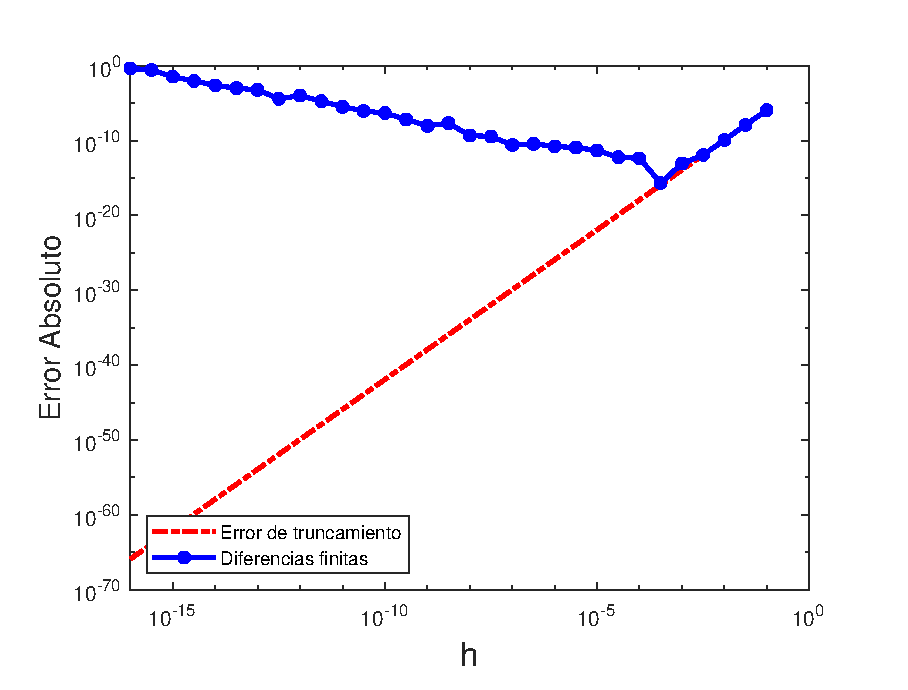
\includegraphics[width=0.65\linewidth]{Gráficas/P5-2.eps}
    \caption{P5-2}
    \label{figcoyoyoyo}
\end{figure}

\subsection*{Problema6}
Repaso de notación \( O \) mayúscula y \( o \) minúscula de una función. Si \( f(x) = O(x^2) \), \( g(x) = O(x^3) \) y \( h(x) = O(x^3) \) cuando \( x \to 0 \), ¿cuáles de las siguientes afirmaciones son verdaderas? Justifique sus respuestas.

\begin{itemize}
    \item[(a)] \( f(x) = o(x) \) cuando \( x \to 0 \)
    \begin{solution}
        Cuando $x\to 0$, existe $M>0$ tal que $|f(x)|\leq M|x^2|$, como $x\neq 0$, tenemos que $\left|\dfrac{f(x)}{x}\right|\leq M|x|$, Luego $\displaystyle\lim_{x\to 0}\left|\frac{f(x)}{x}\right|\leq 0.$ Por el valor absoluto y su continuidad, concluimos que $$\lim_{x\to 0}\frac{f(x)}{x}= 0.$$ Es decir $f(x)=o(x)$ cuando $x\to 0.$ Así la afirmación es \textbf{Verdadera.}
    \end{solution}
    \item[(b)] \( f(x) = o(x^2) \) cuando \( x \to 0 \)
    \begin{solution}
    Sea $f(x)=x^2$, es claro que cuando $x\to 0,$ $f(x)=O(x^2)$ Ahora note que $\dfrac{f(x)}{x^2}=1.$ Por lo tanto
    $$\lim_{x\to 0}\frac{f(x)}{x^2}=1.$$
    Es decir que $f(x)\neq o(x^2).$ Así la afirmación es \textbf{Falsa.}
    \end{solution}
    \item[(c)] \( f(x) \cdot g(x) = O(x^5) \) cuando \( x \to 0 \)
    \begin{solution}
        Cuando $x\to 0$ por hipótesis, existen $M,N>0,$ tales que $|f(x)|\leq M|x^2|$ y $|g(x)|\leq N|x^3|.$ Al ser cantidades positivas, la desigualdad se mantiene si las multiplicamos, es decir
        $$|f(x)||g(x)|\leq (M|x^2|)(N|x^3|).$$
        Si tomamos $K=MN>0,$ tenemos que $|f(x)g(x)|\leq K|x^5|,$ cuando $x\to 0.$ POr lo que $f(x)g(x)=O(x^5).$ Así la afirmación es \textbf{Verdadera.}
        
    \end{solution}
    \item[(d)] \( f(x) + g(x) = O(x^3) \) cuando \( x \to 0 \)
    \begin{solution}
        Sean $f(x)=x^2$ y $g(x)=x^3$, es claro que cuando $x\to 0,$ $f(x)=O(x^2)$ mientras que $g(x)=O(x^3).$ Supongamos que la afirmación es cierta. Luego existe $M>0$ tal que
        $$|x^2+x^3|\leq M|x^3|.$$
        Así 
        $$\left|\frac{1}{x}+1\right|\leq M$$
        Pero como esto se tiene cuando $x\to 0$, el lado derecho eventualmente se hará mas grande que cualquier constante fija. Por lo tanto $f(x)+g(x)\neq O(x^3).$ Asi la afirmación es \textbf{Falsa.}
    \end{solution}
    \item[(e)] \( g(x) - h(x) = 0 \)
    \begin{solution}
        Sean $g(x)=2x^3$ y $h(x)=x^3.$ es claro que ambas son $O(x^3)$ cuando $x\to 0$ pero claramente
        $$2x^3-x^3=x^3\neq 0,$$
        siempre que $x\neq 0.$ que es el caso. Así la afirmación es \textbf{Falsa.}
    \end{solution}
    \item[(f)] \( \dfrac{g(x)}{h(x)} = O(1) \) cuando \( x \to 0 \)
    \begin{solution}
        Sean $g(x)=x^3$ y $h(x)=x^4.$ Para $0<|x|<1$ tenemos que $|x^4|\leq |x^3|$, luego cuando $x\to 0,$ tenemos que $g(x)=O(x^3)$ y $h(x)=O(x^3).$ Supongamos que la afirmación es cierta. En ese caso tendríamos que existe $M>0$ tal que
        $$\left|\frac{1}{x}\right|=\left|\frac{x^3}{x^4}\right|\leq M.$$
        Luego cuando $x\to 0$ en algún punto el lado izquierdo sera mas grande que alguna constante fija, una contradicción. Mostrando así que $\dfrac{g(x)}{h(x)}\neq O(1).$ Así la afirmación es \textbf{Falsa.}
    \end{solution}
\end{itemize}
\end{document}

|